% !TEX root = ../final-main.tex
\chapter{Enhancement-Mode Iteration 3}
\label{ch:iteration-3}

\section{Iteration 3 Process Changes}

The third enhancement-mode iteration was designed to address the main process
limitation identified in Chapter~\ref{ch:iteration-2}: insufficient control of
the recess depth during wet etching. The revised gate geometry from Iteration 2
was retained, since the unrecessed control devices had demonstrated improved
pinch-off and stronger electrostatic control of the mesa channel.

\vspace{1mm}

Four quadrants were processed in this iteration, with two target
recess depths repeated across two samples. Both samples used the same pair of recess
etch times, so that the effect of the gate stack could be separated from the
effect of recess depth. One sample used the recessed Schottky gate process
without an oxide layer, while the second sample included an oxide layer before
gate formation. This allowed the oxide process to be assessed as a possible
method for suppressing the gate leakage observed in Iteration 2.

\vspace{1mm}

For each target depth, the oxide and non-oxide quadrants were etched together.
This was done to ensure that each pair experienced the same etchant condition,
timing, agitation, and handling. The intention was to produce two recess depths
on each sample, while keeping the oxide and non-oxide comparison as direct as
possible.

\begin{table}[htbp]
  \centering
  \caption{Iteration 3 sample matrix used to compare recess etch time and
  gate-oxide inclusion.}
  \label{tab:iteration3-quadrants}
  \begin{tabular}{c c c}
    \hline
    Sample & Gate stack & Recess Etch Time \\
    \hline
    1 & No Gate Oxide & \SI{45}{\second} \\
    1 & No Gate Oxide & \SI{60}{\second} \\
    2 & Gate Oxide& \SI{45}{\second} \\
    2 & Gate Oxide & \SI{60}{\second} \\
    \hline
  \end{tabular}
\end{table}

\section{Pilot Etch Calibration}

The key process modification in Iteration 3 was the use of a pilot sample immediately
before processing the device quadrants. The pilot sample was patterned with a
series of strip features in the photoresist and measured using the AlphaStep after etching. 
This provided a direct check of the etch rate for the specific etchant condition used
for the device run, rather than relying only on the earlier incremental
calibration curves.

\vspace{1mm}

The pilot sample was etched for \SI{60}{\second}, which was predicted to place
the recess depth close to the intended \SIrange{25}{30}{\nano\metre} range. The
measured depth was approximately \SI{34}{\nano\metre}. Although this was
slightly deeper than the nominal target, it was much closer to the required
range than the excessive depth observed in Iteration 2. This gave sufficient
confidence to proceed with the device etches.

\vspace{1mm}

The device samples were then etched using two timings. One oxide/non-oxide pair
was etched for \SI{45}{\second}, while the second pair was etched for
\SI{60}{\second}, matching the pilot sample. The aim was not to produce a large
depth separation, but to create two controlled recess conditions within the
range expected to shift the threshold voltage into enhancement-mode operation.

\section{Fabrication and Optical Inspection}

After the recess etches, the gate lithography process was carried out using the
same gate geometry as Iteration 2. During development of the gate-formation
photoresist, an unexpected surface effect was observed. The recessed regions
showed a pinholing pattern across the etched areas. This had not been observed
in the earlier iterations, but it appeared consistently across the four etched
quadrants processed in Iteration 3.

\vspace{4mm}

\begin{figure}[htbp]
  \centering
  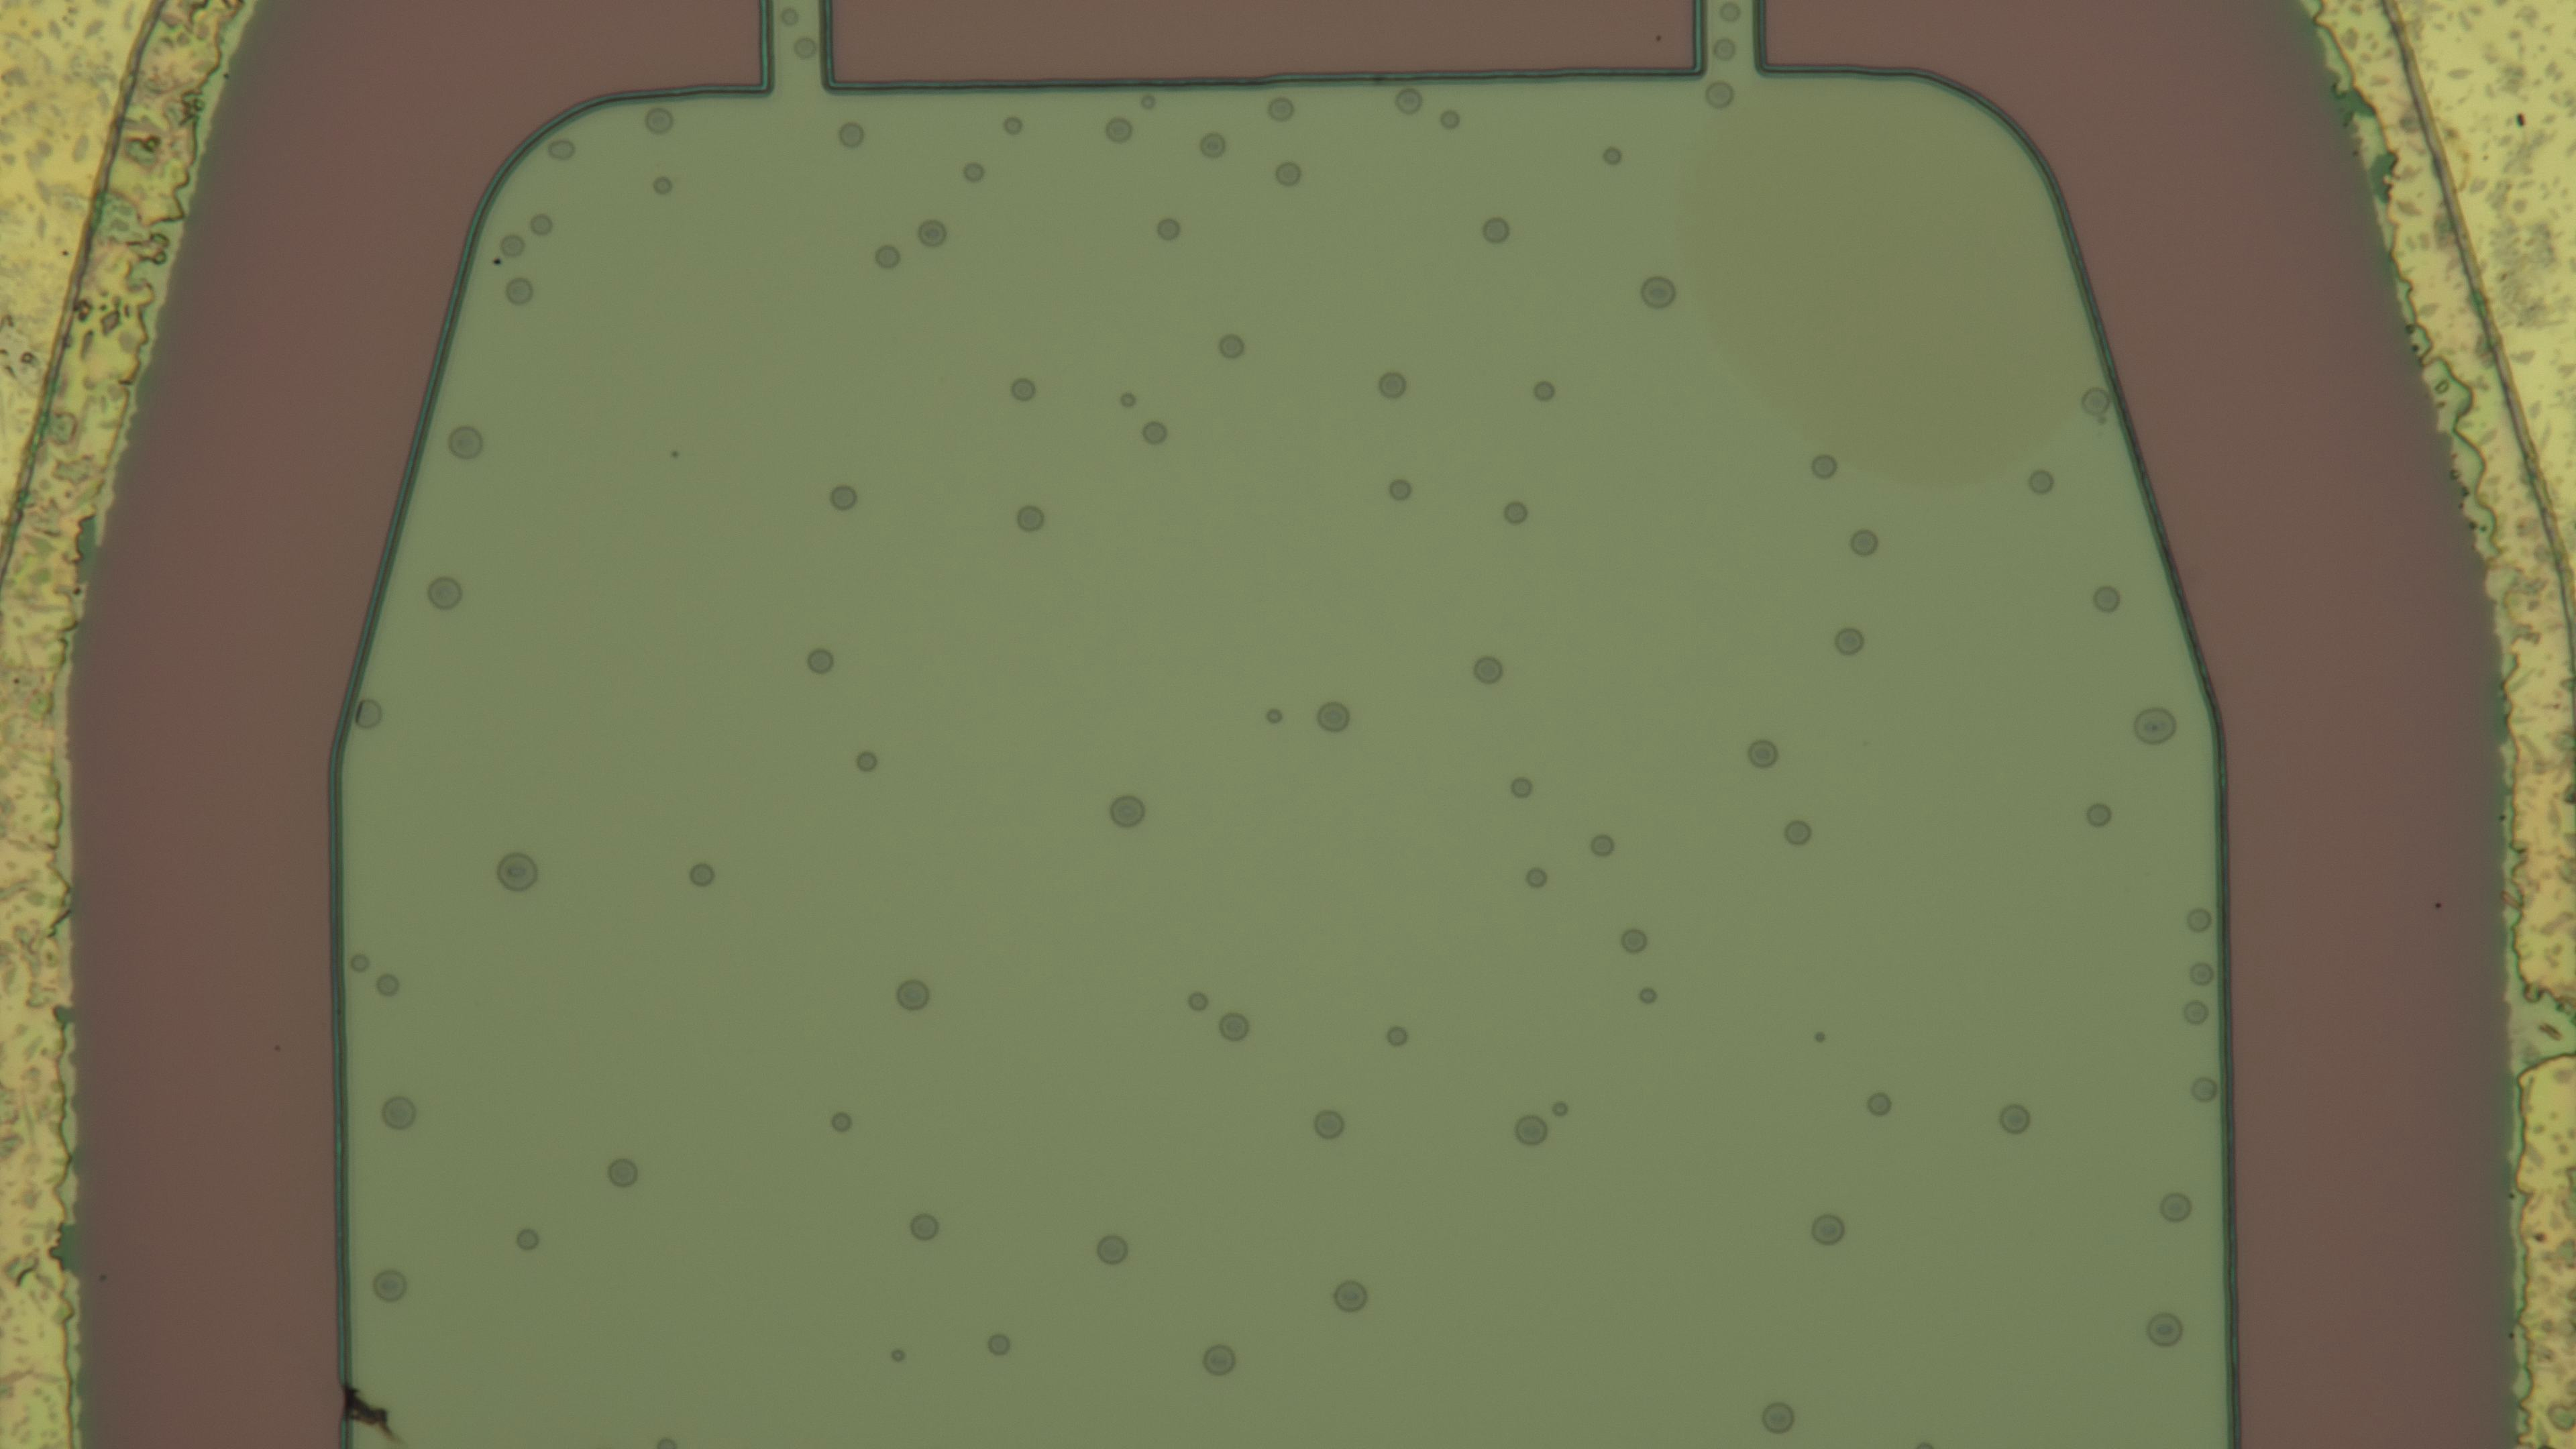
\includegraphics[width=0.78\linewidth]{figures/fabrication_images/enhancement_mode_images/iteration3/sample2_q4_x50_holes_1.jpg}
  \caption{Optical microscopy of the developed gate-recess region on the oxide
  sample.}
  \label{fig:iteration3-algaas-pitting}
\end{figure}

\vspace{1mm}

This pattern is believed to result from the MF-351 developer attacking the
exposed AlGaAs surface after the recess etch. MF-351 is an NaOH-based
developer, and the corresponding AZ 351B developer family is reported to attack
aluminium-containing surfaces \cite{AZ351BData}. The
aluminium in AlGaAs undergoing alkaline dissolution, with OH$^{-}$
ions forming soluble aluminate species such as $AlOH_4$
\cite{MicroChemicalsDev}. This observation ultimately provided some qualitative
evidence that this time, the recess was located in the AlGaAs layer.

\vspace{1mm}

The gates were formed using the established gate formation process.
Optical inspection confirmed that the completed gates intersected the mesa between source and drain. 
However, the fabrication yield was not perfect. On the non-oxide sample, only seven out of
ten recessed devices were successfully measurable. Several devices were lost
because gate metal did not lift off cleanly in some regions, producing
short-circuit paths between source and drain. The oxide sample showed cleaner
lift-off in the inspected devices, as shown in Figure~\ref{fig:iteration3-liftoff}.

\begin{figure}[htbp]
  \centering
  \begin{subfigure}{0.48\linewidth}
    \centering
    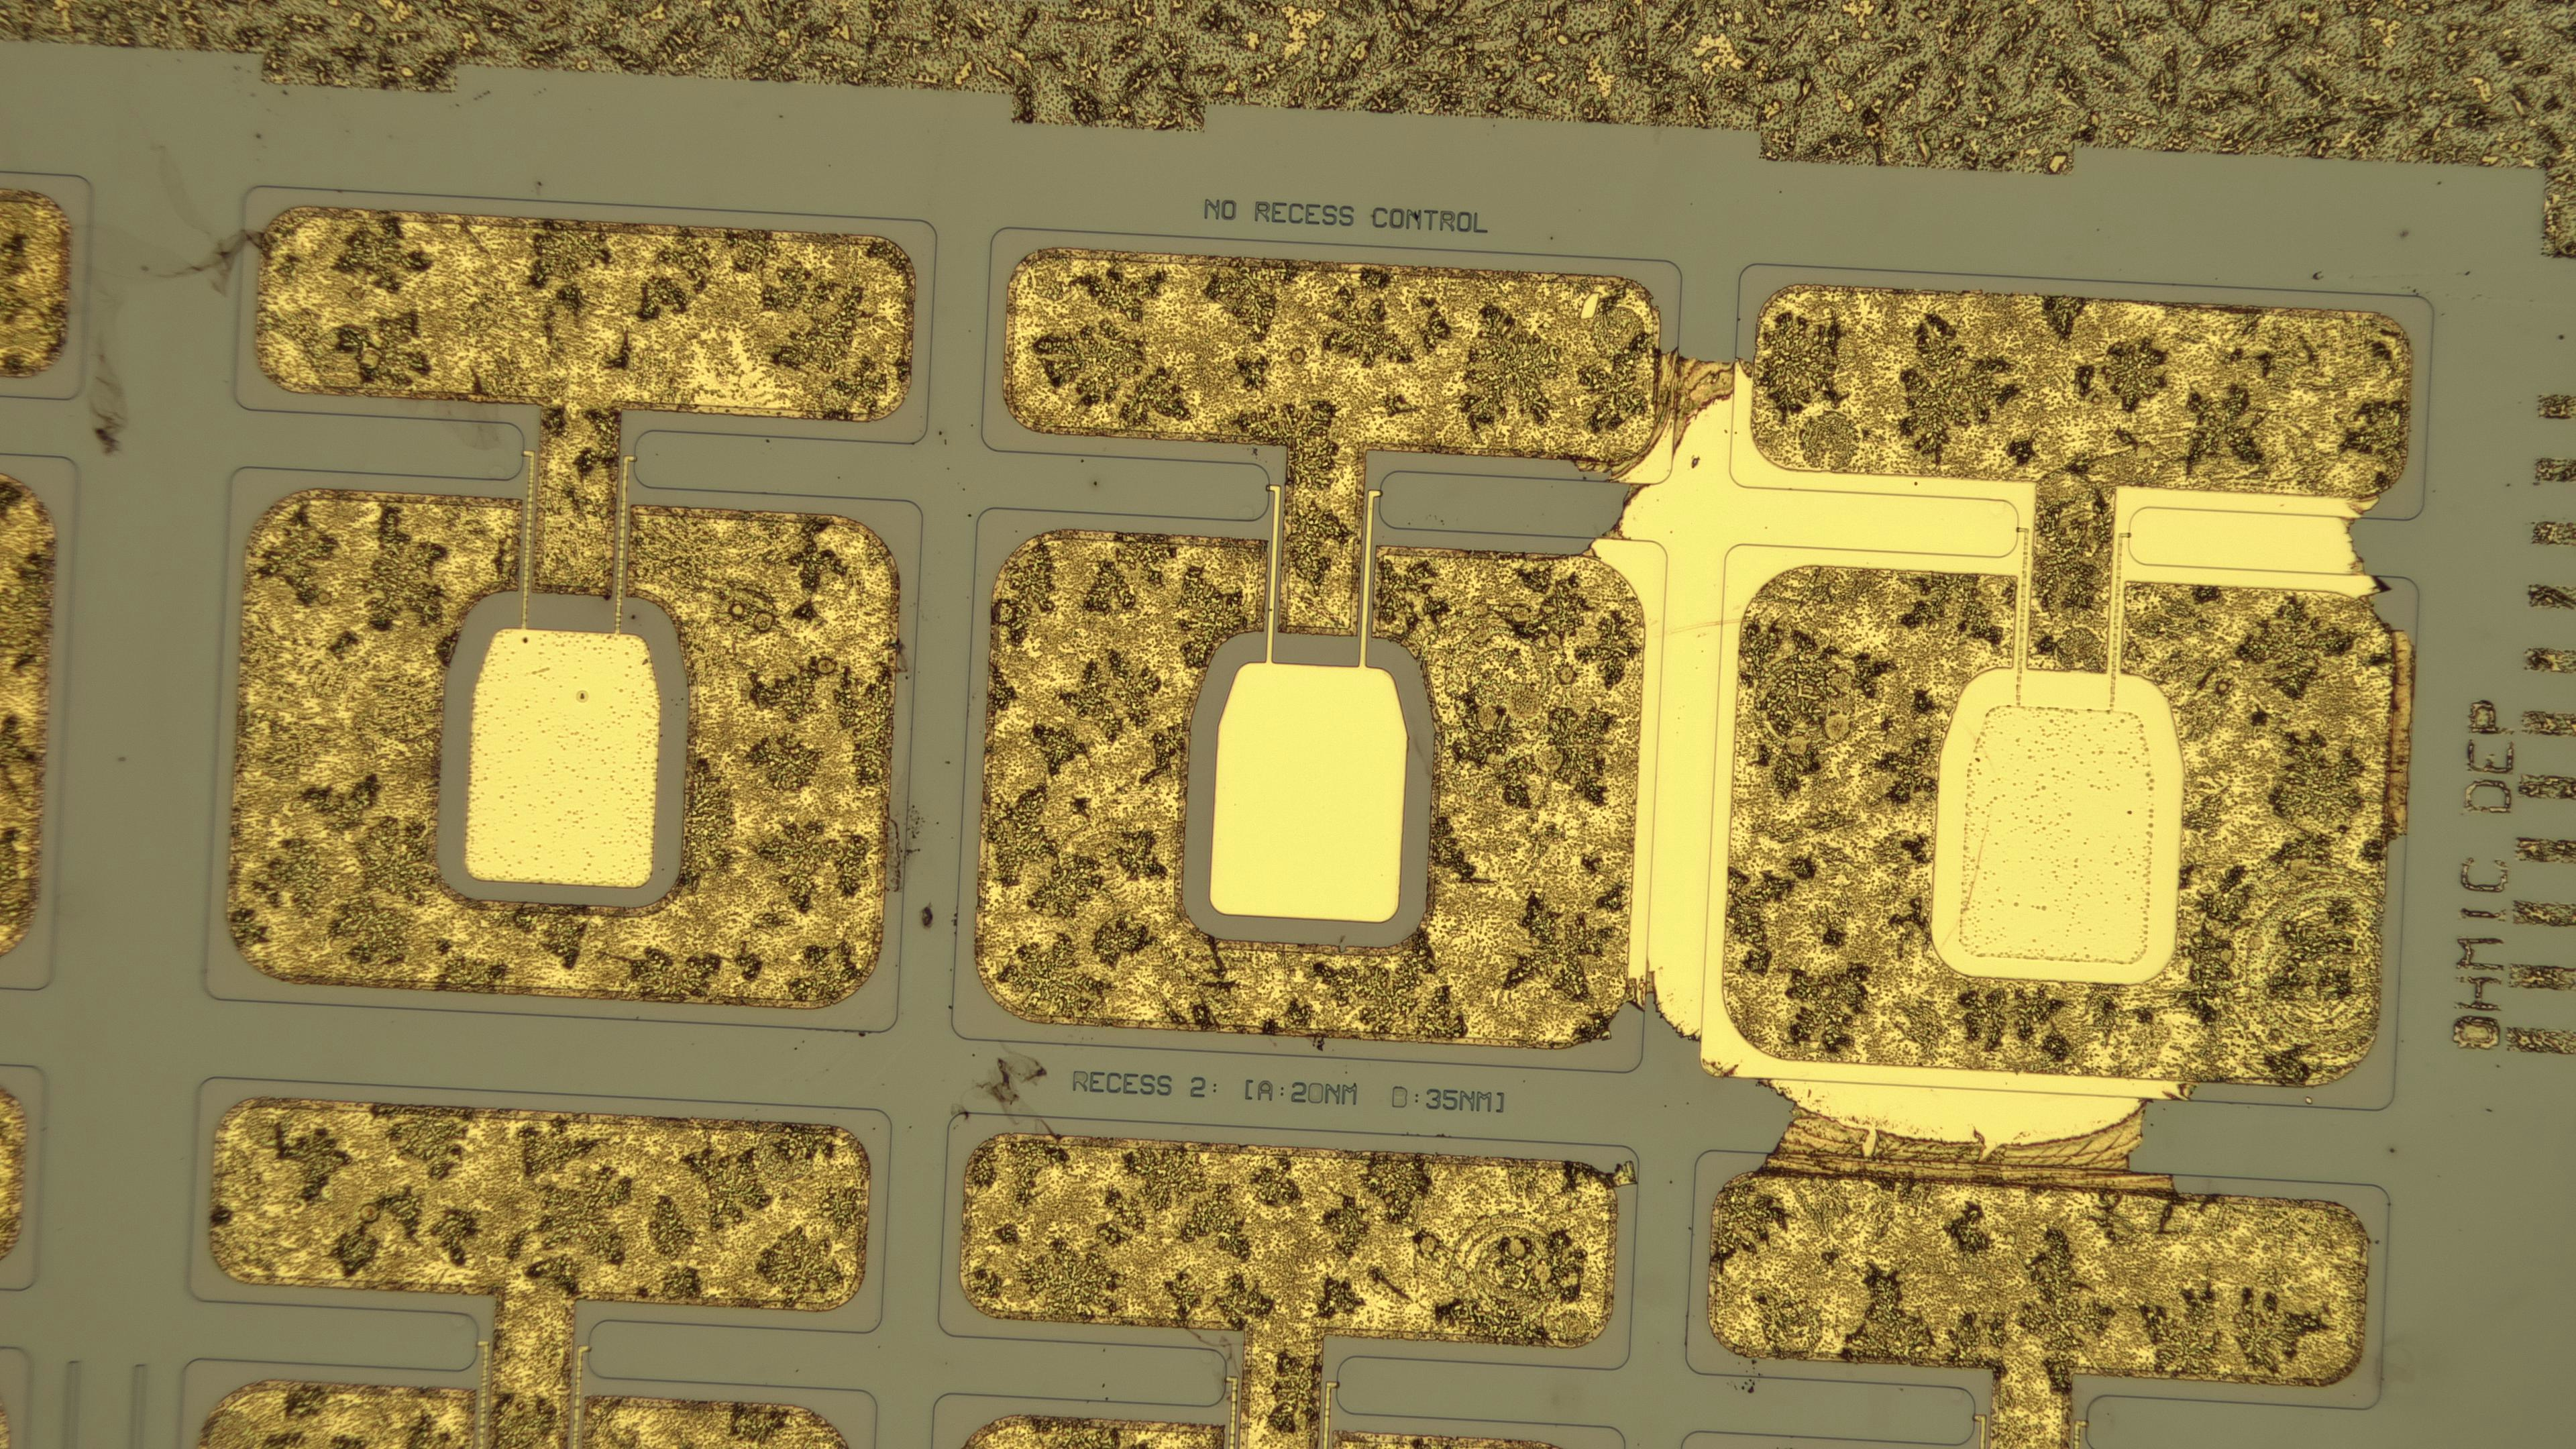
\includegraphics[width=\linewidth]{figures/fabrication_images/enhancement_mode_images/iteration3/sample1_q1_bad_liftoff.jpg}
    \caption{Poor lift-off on non-oxide sample 1.}
  \end{subfigure}
  \hfill
  \begin{subfigure}{0.48\linewidth}
    \centering
    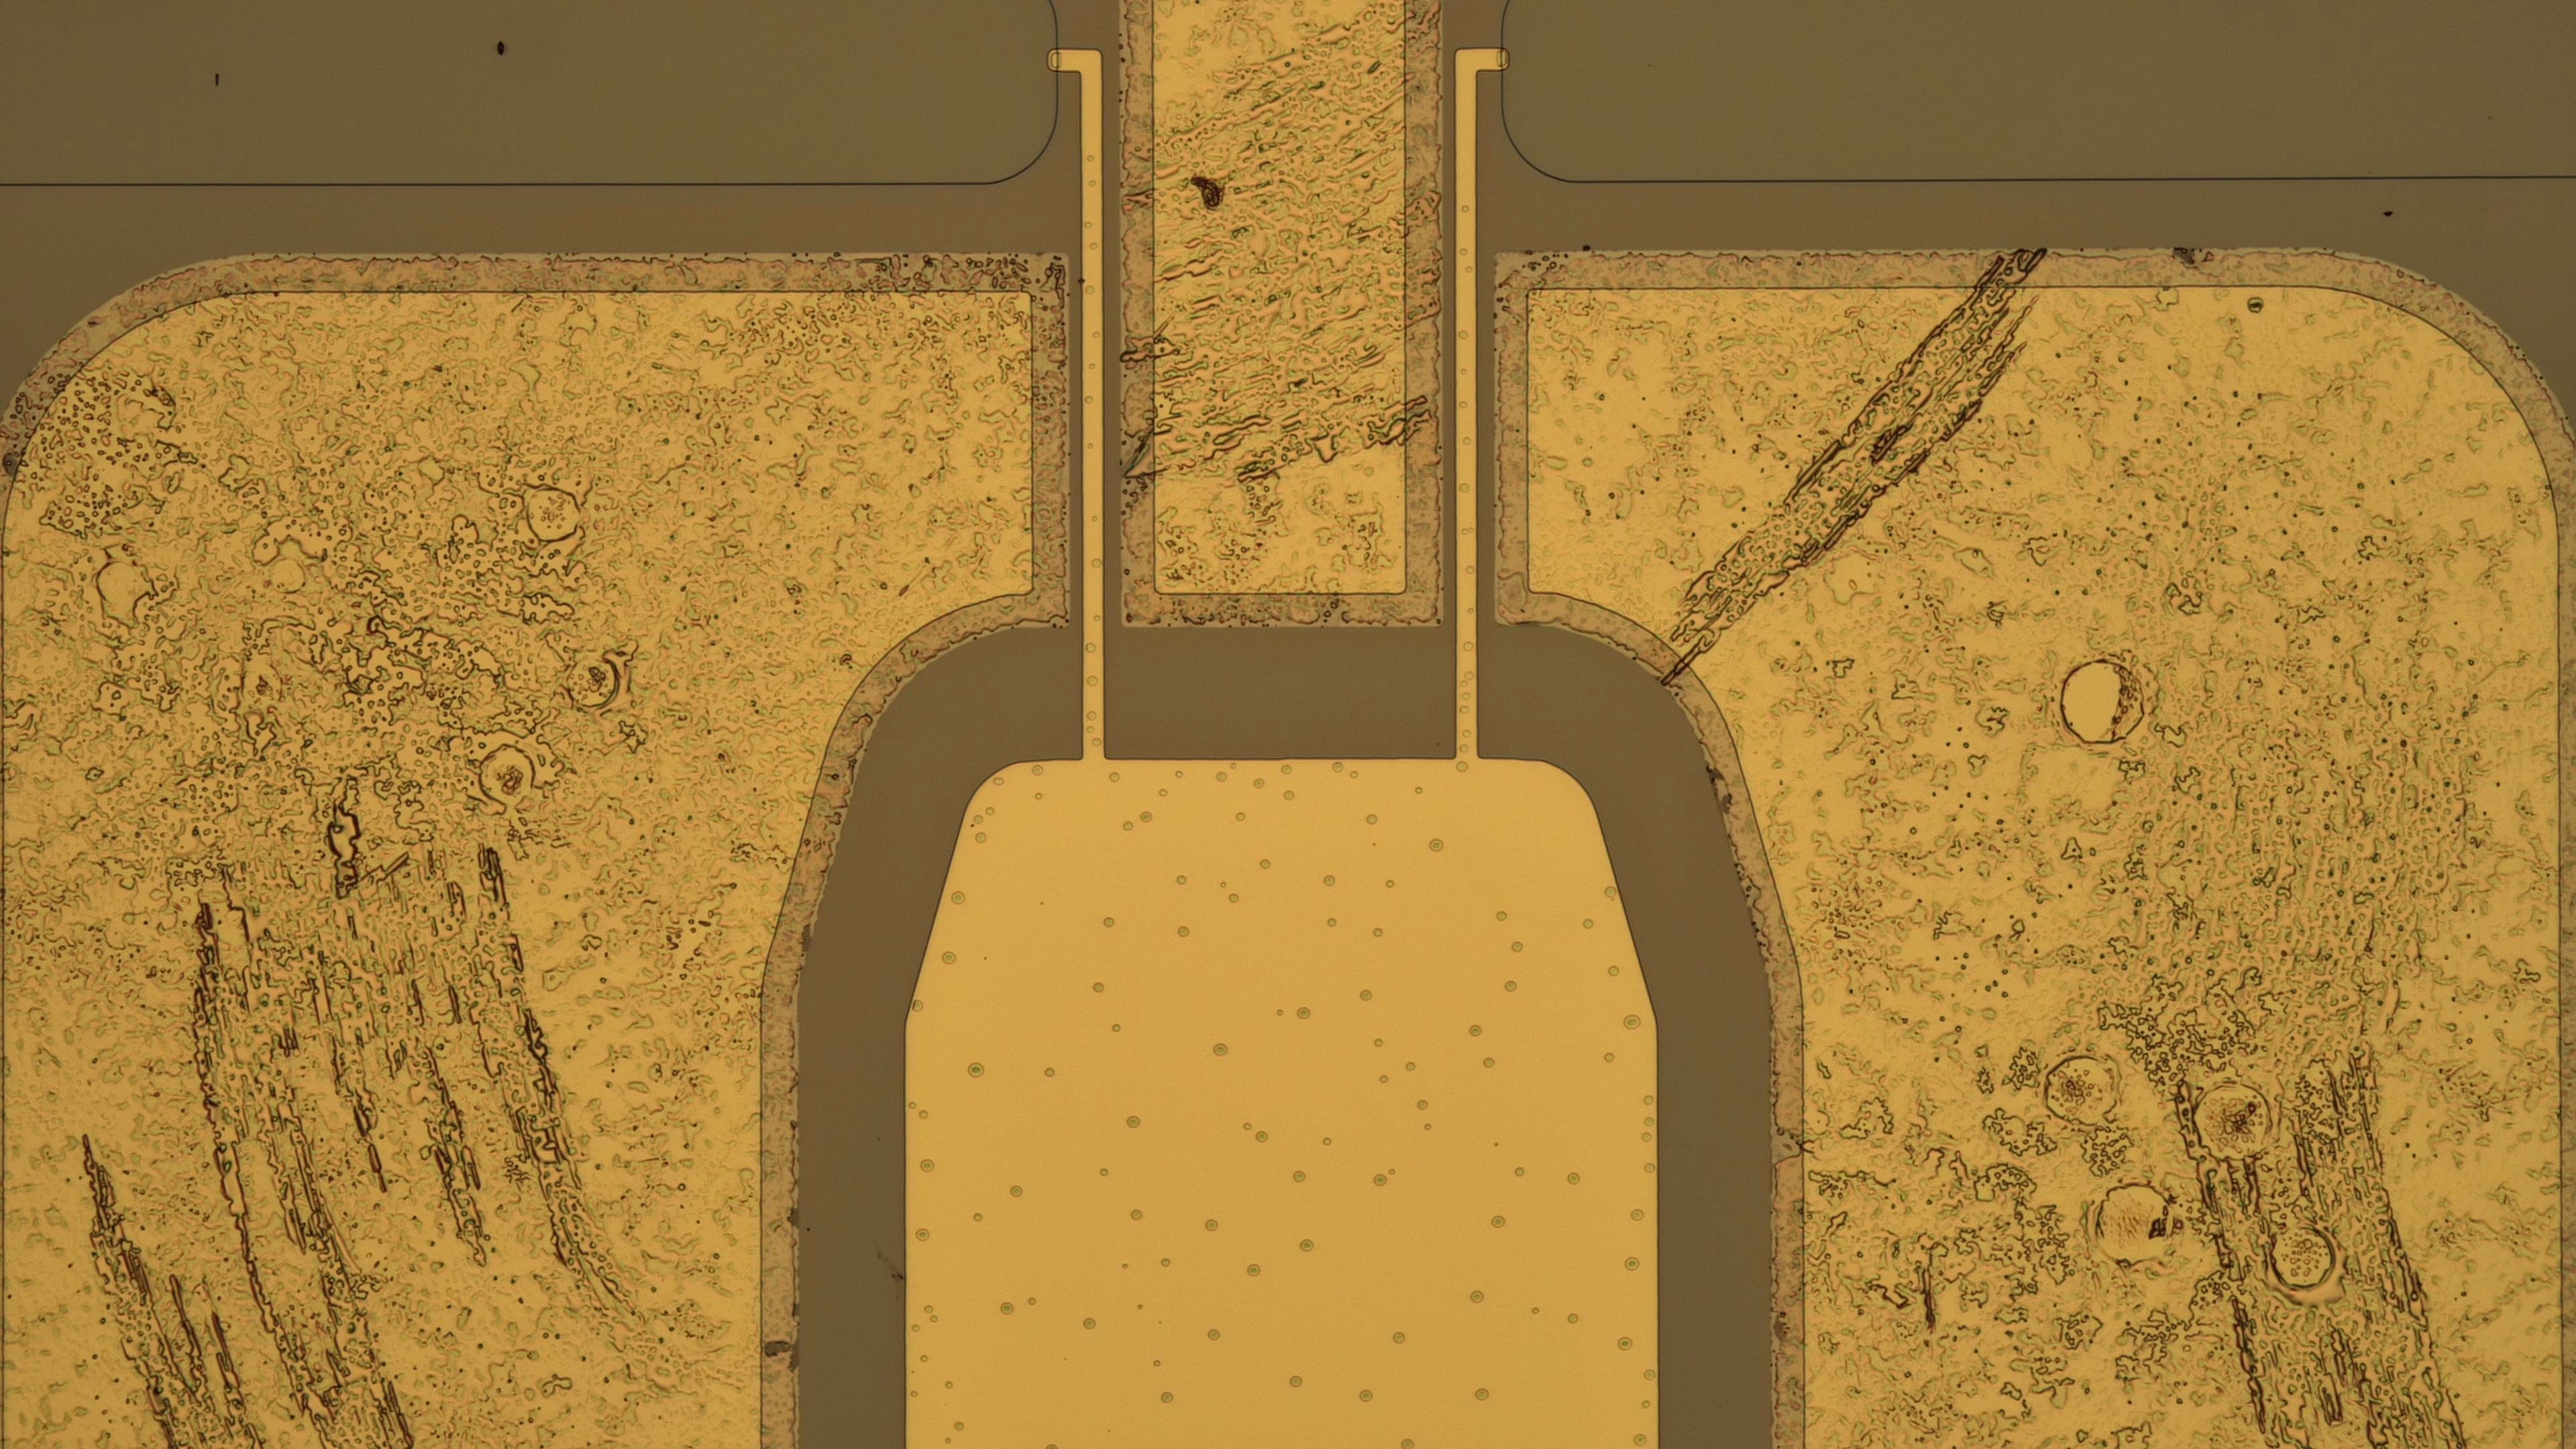
\includegraphics[width=\linewidth]{figures/fabrication_images/enhancement_mode_images/iteration3/sample2_q4_x20_liftoff.jpg}
    \caption{Cleaner lift-off on oxide sample 2.}
  \end{subfigure}
  \caption{Optical microscopy comparison of Iteration 3 gate metal lift-off.}
  \label{fig:iteration3-liftoff}
\end{figure}

\begin{figure}[htbp]
  \centering
  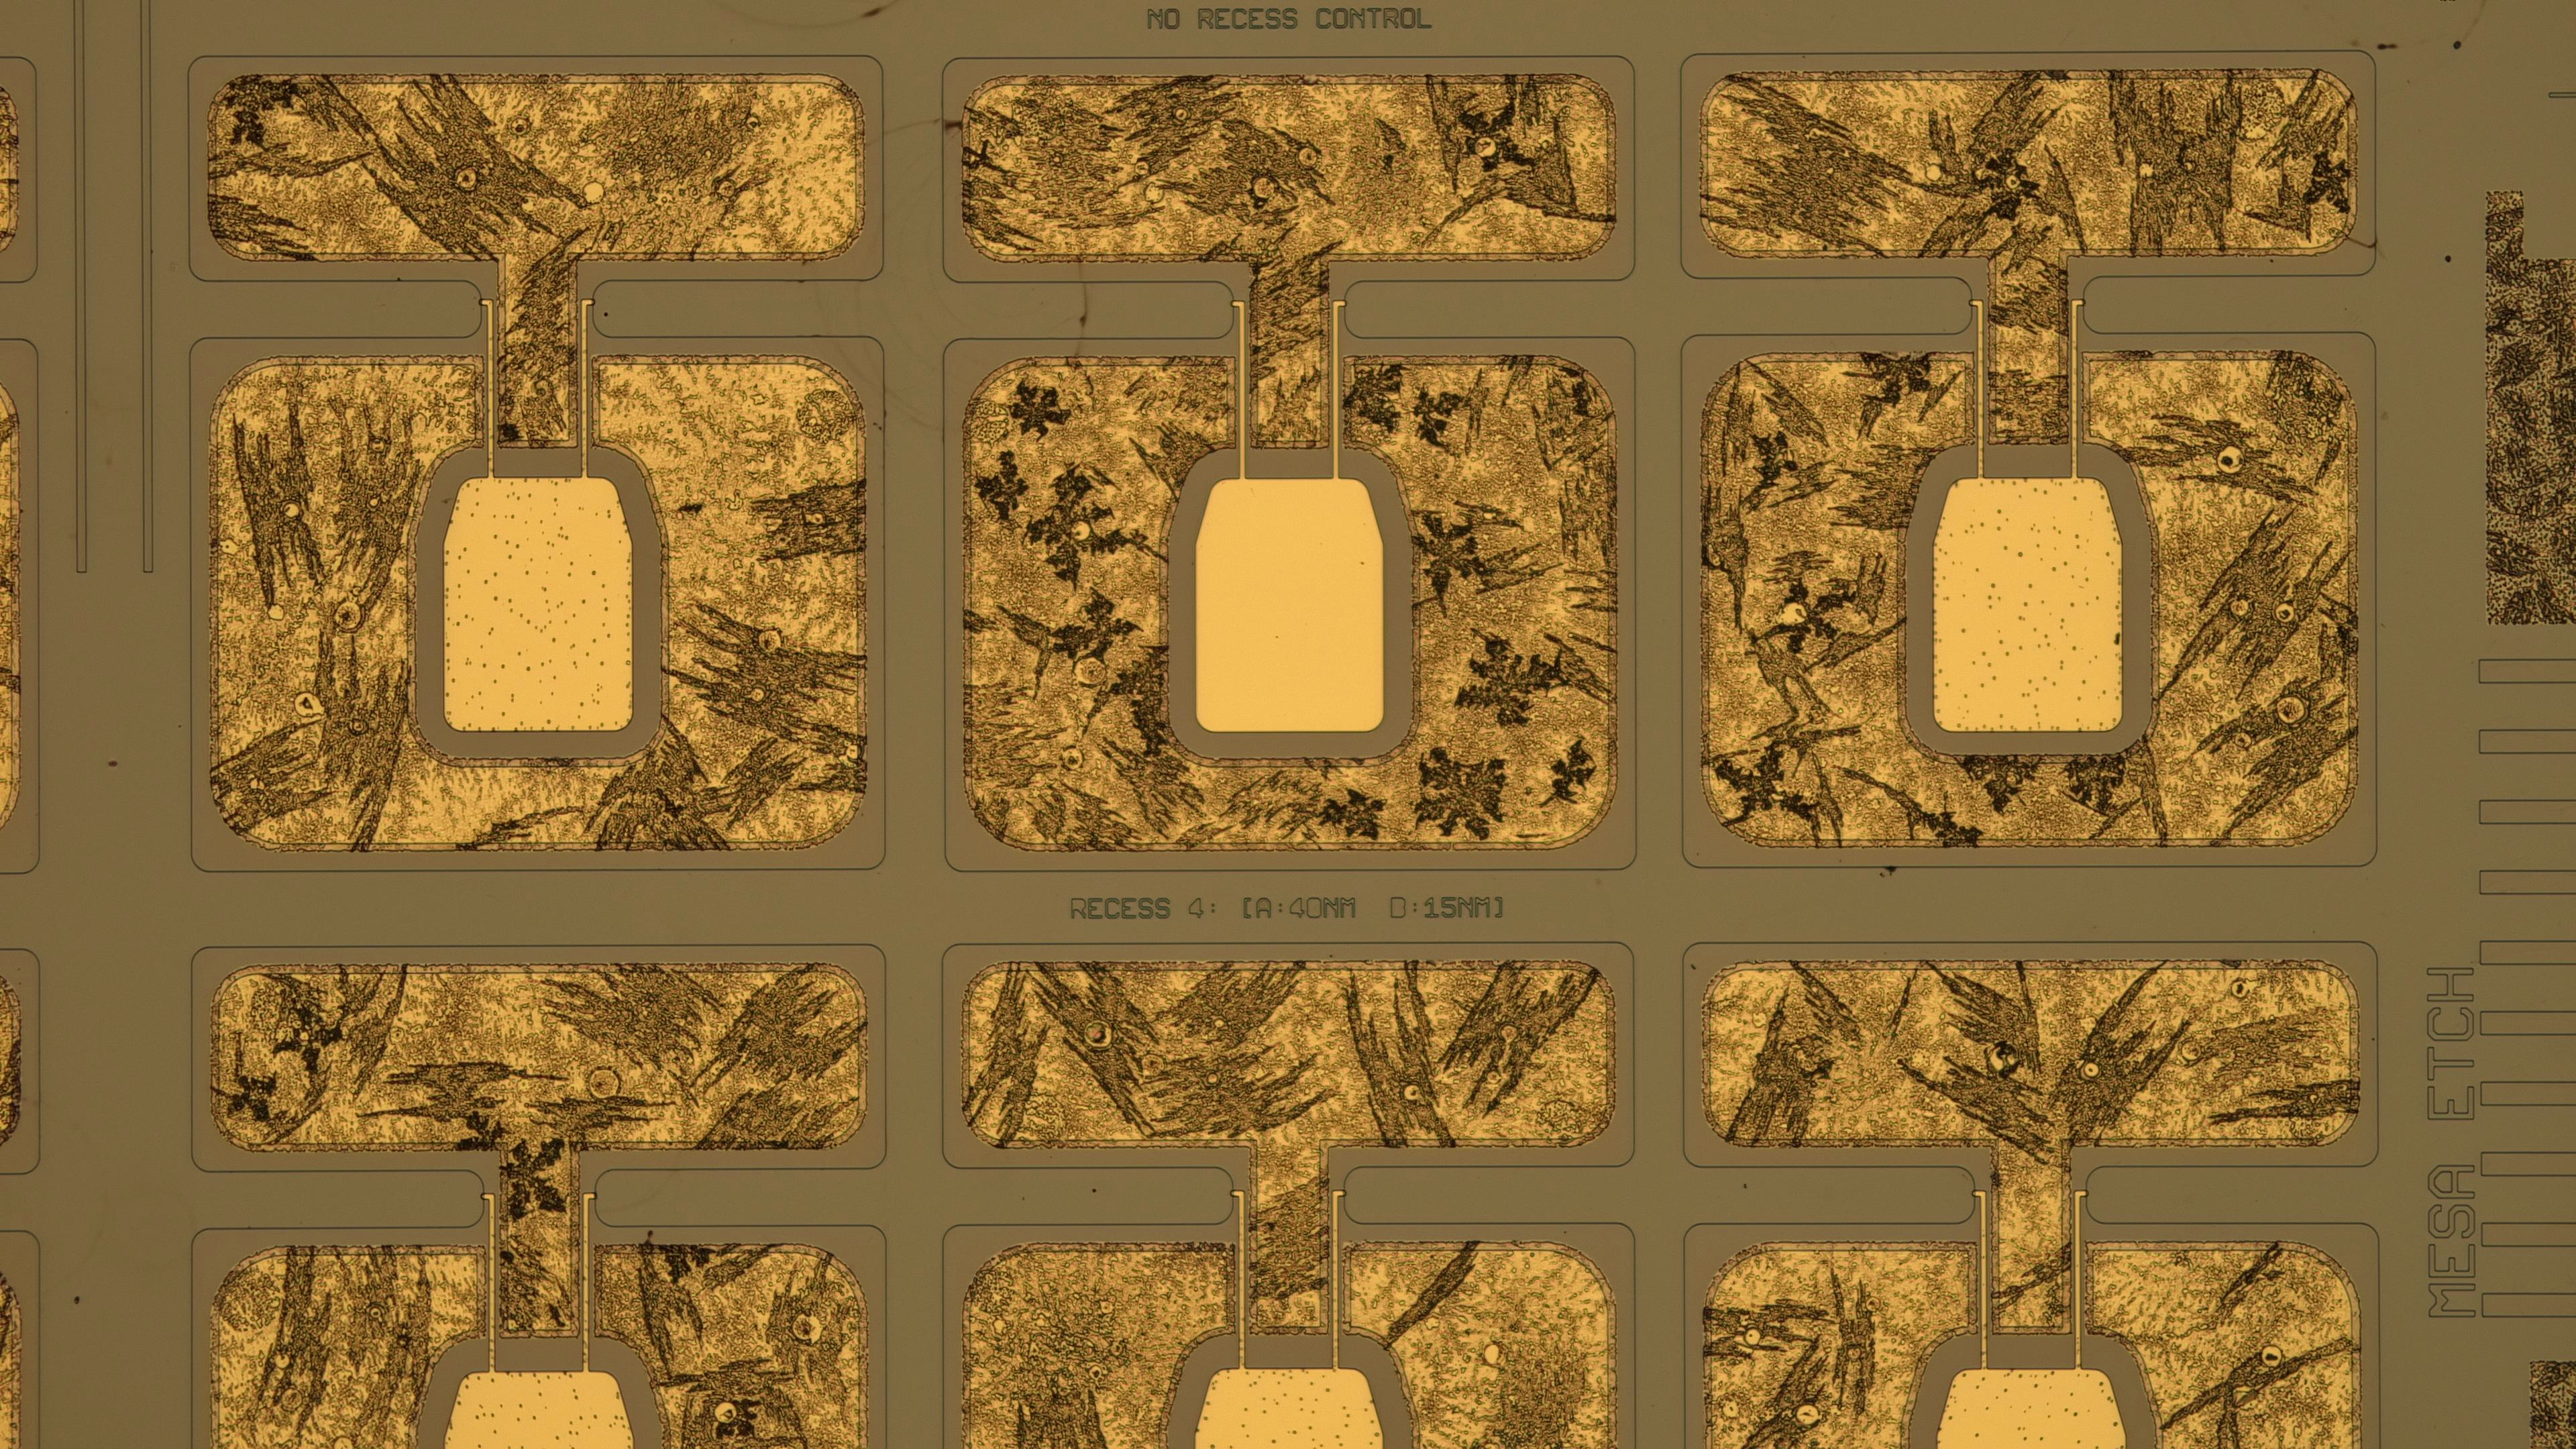
\includegraphics[width=1\linewidth]{figures/fabrication_images/enhancement_mode_images/iteration3/sample2_q4_x5_liftoff.jpg}
  \caption{Low-magnification optical microscopy of a completed Iteration 3
  oxide quadrant.}
  \label{fig:iteration3-device-overview}
\end{figure}


\section{Electrical Results}

\subsection{Non-Oxide Recessed Devices}

The main successful result from Iteration 3 was obtained from the non-oxide
recessed devices. Unlike the recessed devices in Iteration 2, these devices
functioned as enhancement-mode transistors. This indicates that the recess was
now sufficiently deep to shift the threshold voltage positive, but not so deep
that the conducting channel was completely removed.

\begin{figure}[htbp]
  \centering
  \makebox[\linewidth][c]{\hspace*{-0.04\linewidth}
\includegraphics[width=0.9\linewidth]{figures/electrical_analysis/enhancement_mode/iteration_3/gate_transfer.png}}
  \caption{Gate-transfer characteristics for the Iteration 3 non-oxide recessed
  devices and unrecessed control.}
  \label{fig:iteration3-nonoxide-transfer}
\end{figure}

\vspace{1mm}

The \SI{45}{\second} recessed device showed a positive threshold voltage of
approximately \SI{0.8}{\volt}, while the \SI{60}{\second} recessed device showed
a more positive threshold voltage of approximately \SI{1.5}{\volt}. This demonstrated the key
trend; the longer recess etch produced a larger positive shift in
threshold voltage.

\vspace{1mm}

The drain-source current was also reduced by the recess process. This is
consistent with the removal of donor material and the corresponding reduction
in carrier density available for conduction. The same effect was observed in
Iteration 1, but the relationship is clearer here because both Iteration 3
recess depths produced functioning enhancement-mode devices. The
\SI{60}{\second} recess showed a slightly lower drain current than the
\SI{45}{\second} recess, consistent with the greater removal of active material.


\vspace{1mm}

These results demonstrate the intended relationship between recess depth and
threshold-voltage shift. Increasing the recess depth moved the threshold
voltage further into the positive gate-bias region, while also reducing the
available drain-source current. This is the central trade-off of the recessed
gate approach: greater recess depth improves normally-off operation, but it also
reduces the remaining channel charge.

\subsection{Oxide Devices}

The oxide sample showed a different electrical response. The recessed oxide
devices did not turn on within the measured gate-voltage range, even at high
positive gate bias. This suggests that the combination of recessing and oxide
deposition suppressed the channel too strongly under the applied measurement
conditions.

\begin{figure}[htbp]
  \centering
  \makebox[\linewidth][c]{\hspace*{-0.04\linewidth}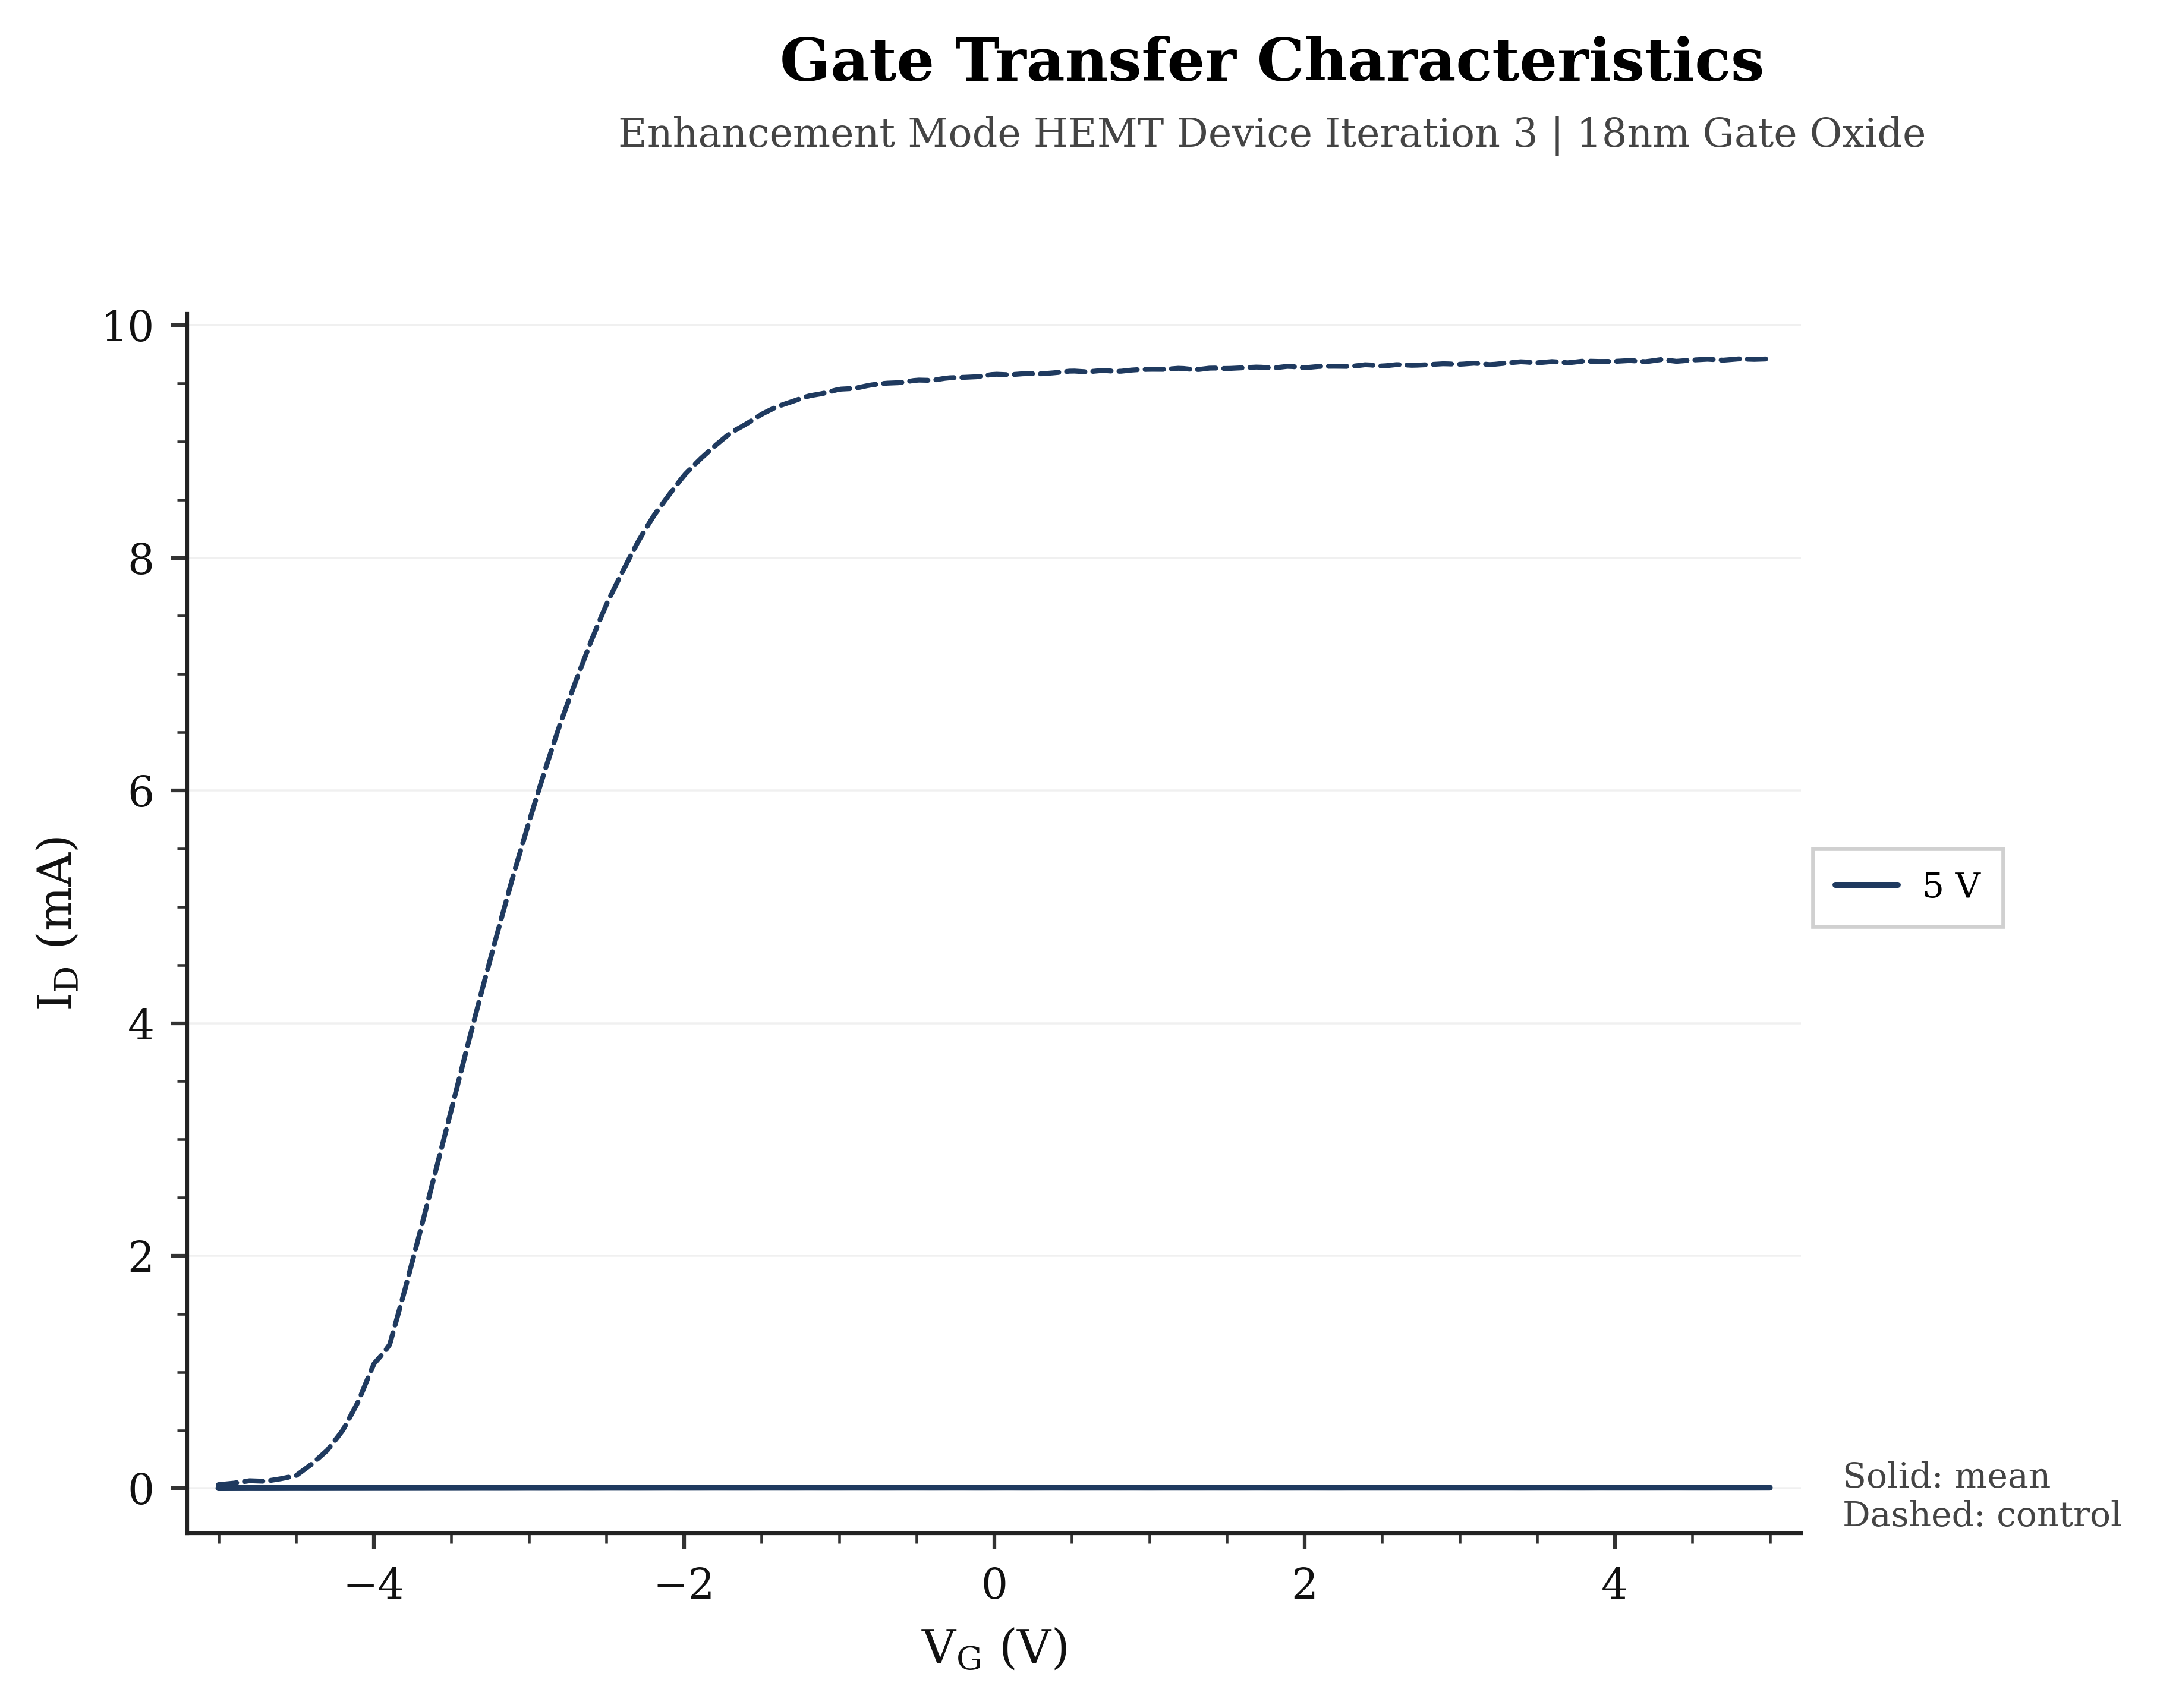
\includegraphics[width=0.88\linewidth]{figures/electrical_analysis/enhancement_mode/iteration_3/gate_oxide_q2_transfer.png}}
  \caption{Gate-transfer comparison for the recessed oxide device and
  unrecessed oxide control.}
  \label{fig:iteration3-oxide-transfer}
\end{figure}

\vspace{1mm}

The unrecessed oxide control device did operate as a depletion-mode HEMT, but
with a substantially more negative threshold voltage of approximately
\SI{-4.2}{\volt}. This indicates that the oxide layer changed the electrostatic
response of the gate stack, even without recessing.

\vspace{1mm}

The major benefit of the oxide process was the gate leakage performance. The
oxide devices showed extremely low gate leakage, on the order of picoamps. This
is a substantial reduction compared with the recessed Schottky-gate leakage
observed in Iteration 2, and confirms that the oxide layer can act as an
effective leakage-suppression layer.

\begin{figure}[htbp]
  \centering
  \makebox[\linewidth][c]{\hspace*{-0.04\linewidth}
\includegraphics[width=0.9\linewidth]{figures/electrical_analysis/enhancement_mode/iteration_3/gate_leakage.png}}
  \caption{Gate-leakage comparison between unrecessed devices with and without
  the oxide layer.}
  \label{fig:iteration3-oxide-leakage-control}
\end{figure}

\begin{figure}[htbp]
  \centering
  \makebox[\linewidth][c]{\hspace*{-0.04\linewidth}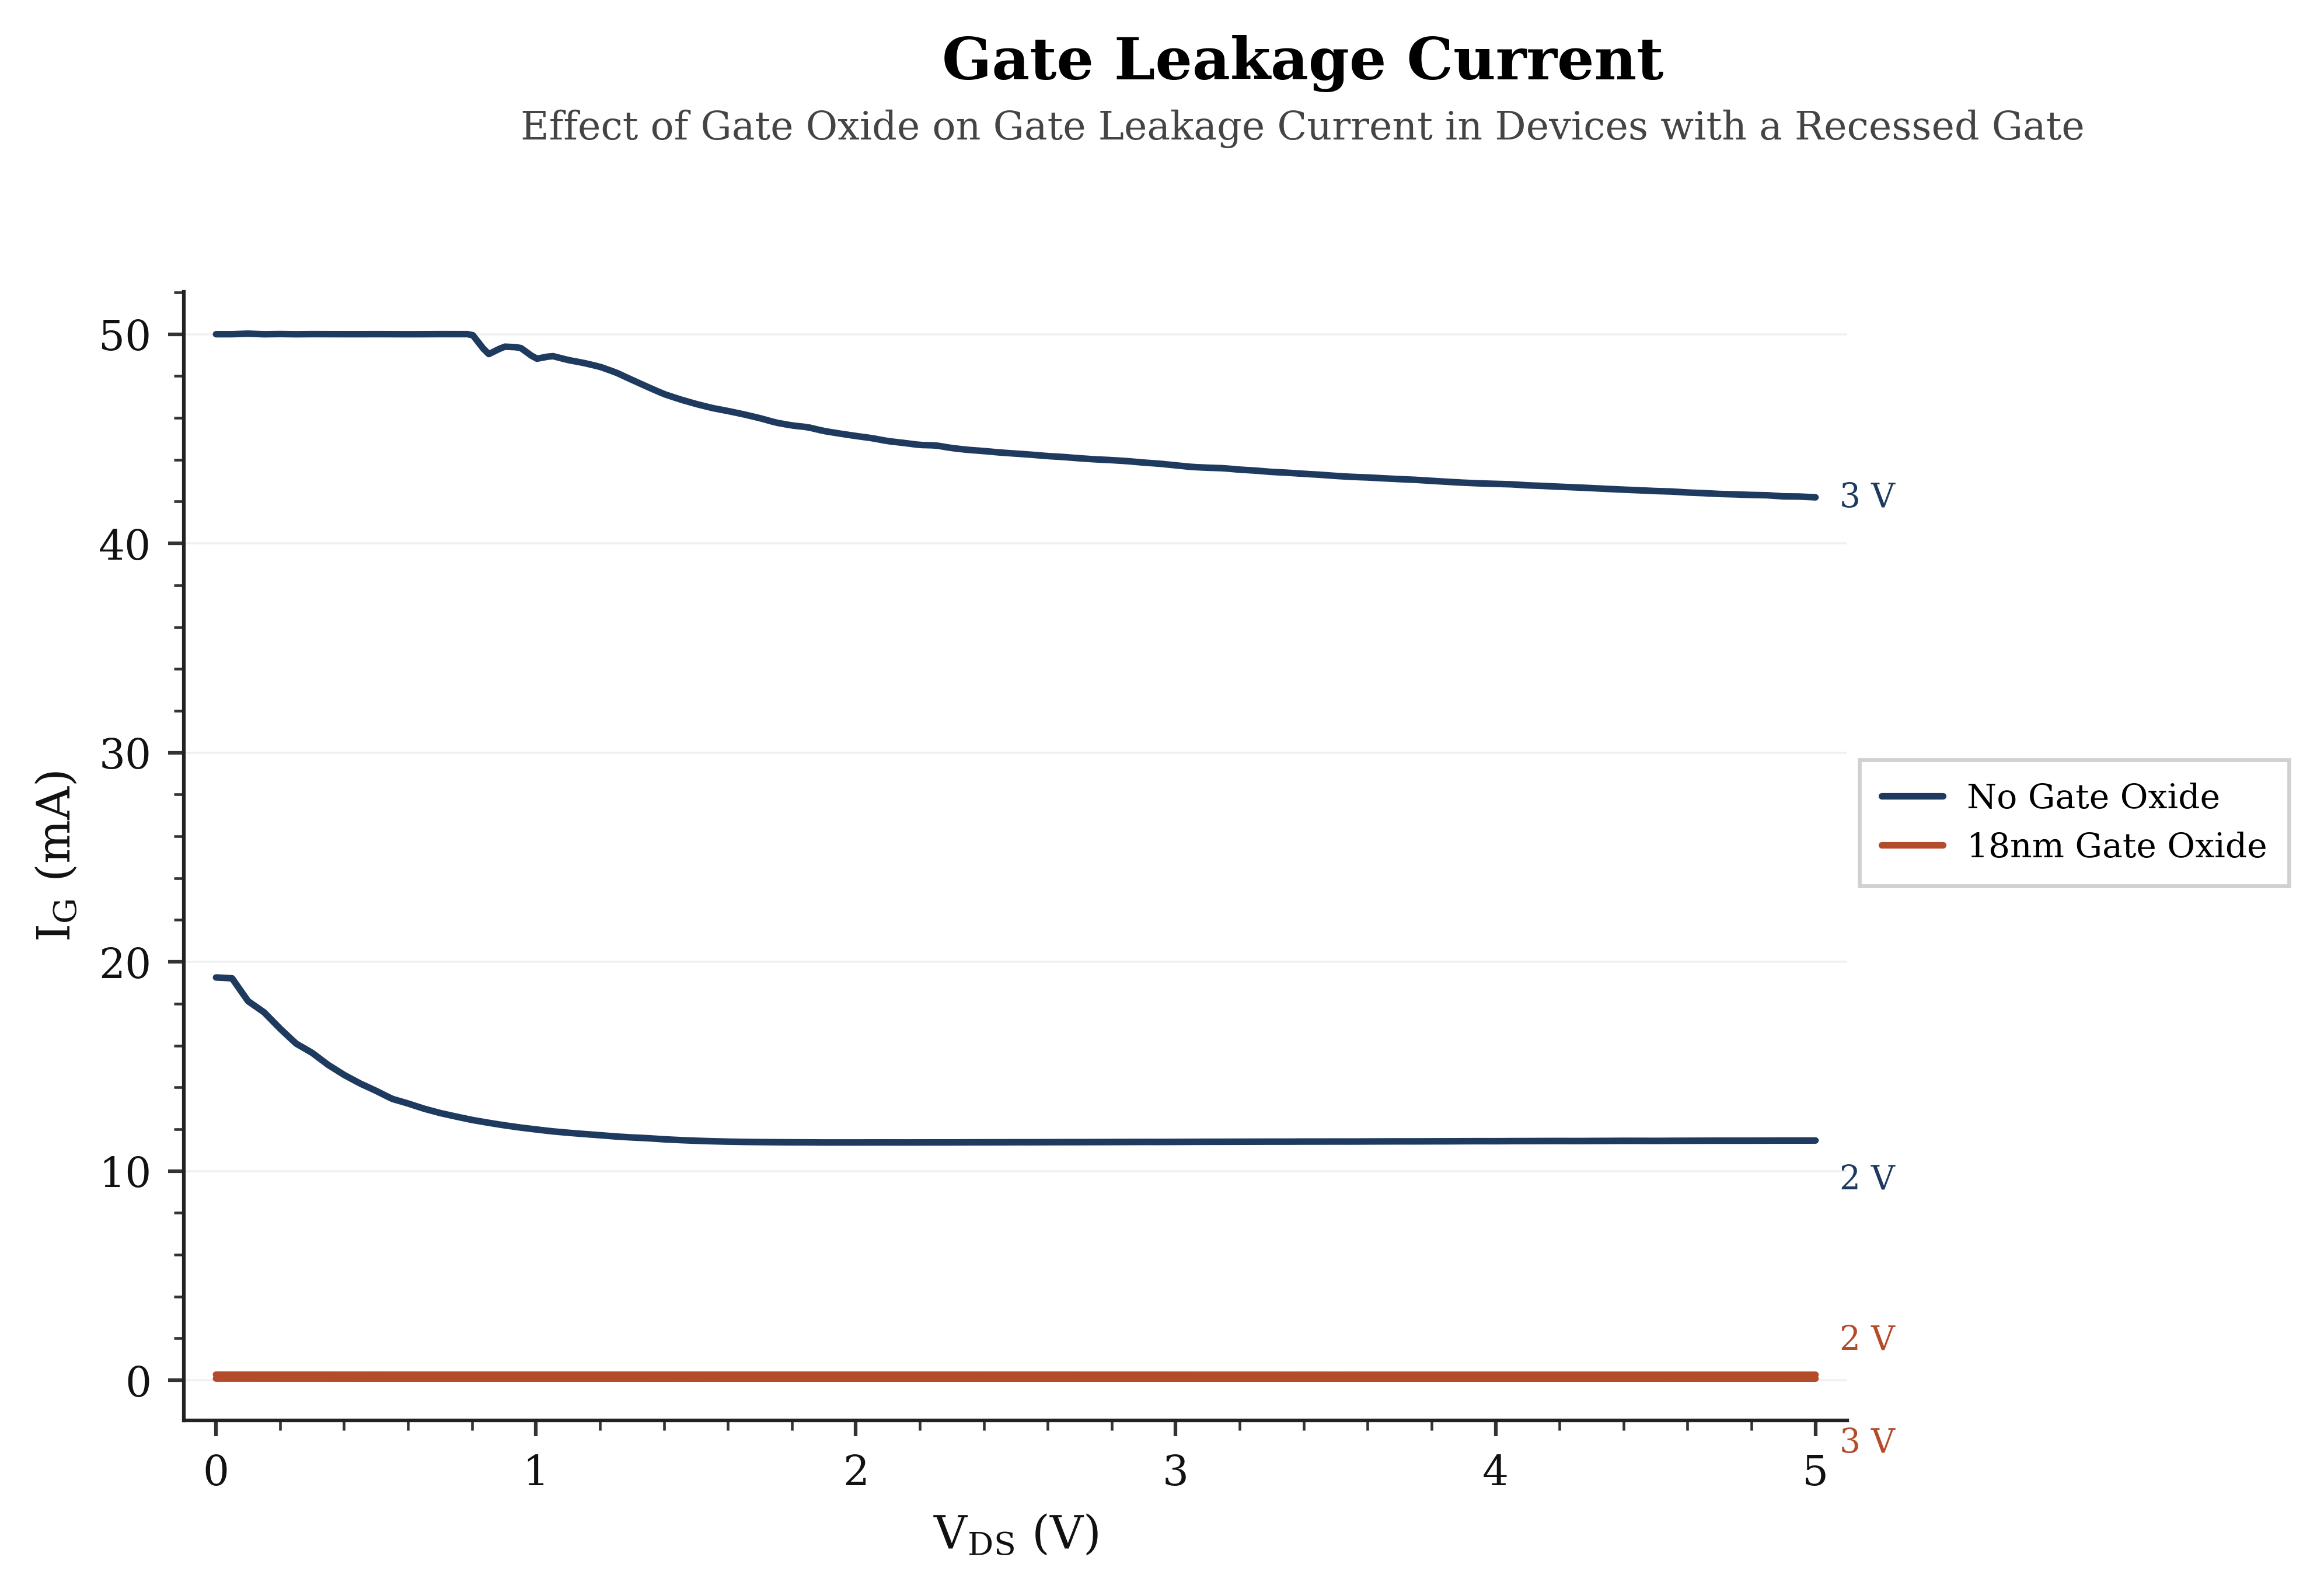
\includegraphics[width=0.9\linewidth]{figures/electrical_analysis/enhancement_mode/iteration_3/gate_leakage_recess.png}}
  \caption{Gate-leakage comparison between recessed Iteration 3 devices with
  and without the oxide layer.}
  \label{fig:iteration3-oxide-leakage-recess}
\end{figure}


\vspace{1mm}

The oxide result therefore represents a different trade-off. The
\SI{18}{\nano\metre} oxide layer increased the physical separation between the
gate metal and the channel surface. For a given applied gate voltage, this
reduces the gate coupling to the channel compared with a direct Schottky gate,
because a larger fraction of the applied bias is dropped across the oxide. In
the unrecessed control device, this changed the threshold voltage but still
allowed depletion-mode operation. In the recessed devices, however, the donor
material had already been partially removed, so the oxide further increased the
gate bias required to recover a conducting channel. The result was excellent
leakage suppression but no functioning transistor
within the tested voltage range.

\section{Analysis}

The introduction of the pilot etch calibration greatly improved confidence in
the recess etch process. As a result, enhancement-mode behaviour was achieved
in the devices without gate oxide.

\vspace{1mm}

The comparison between the \SI{45}{\second} and \SI{60}{\second} non-oxide
devices confirms that the threshold voltage is sensitive to recess depth. The
longer etch produced the more positive threshold voltage, while also reducing
the drain-source current. This is consistent with the expected role of the
donor layer: removing more donor material reduces the electron density in the
channel and shifts the gate voltage required to form a conducting path.

\vspace{1mm}

The pinholing or pitting observed during photoresist development suggests that 
the exposed AlGaAs surface was chemically sensitive to the developer once the cap layer had been removed. 
This did not prevent successful operation in the non-oxide devices, but it is a process concern because surface
damage or roughness may affect leakage, yield, and device repeatability. Different 
photoresist developers should be considered when interpreting the process
limitations.

\vspace{1mm}

The oxide devices confirmed the leakage trade-off identified in
Chapter~\ref{ch:iteration-2}. The oxide layer strongly suppressed gate leakage,
as shown in Figures~\ref{fig:iteration3-oxide-leakage-control}
and~\ref{fig:iteration3-oxide-leakage-recess}, but the recessed oxide devices
did not conduct under the measured conditions. Leakage suppression alone is
therefore not sufficient; the gate stack must also preserve enough
electrostatic access to the channel to allow turn-on at a practical gate
voltage.
